\documentclass[11pt]{article}
\usepackage[margin=1in, top=0in]{geometry}
\usepackage{xcolor}
\usepackage{tikz}
\usepackage{titlesec}
\usepackage[hidelinks]{hyperref}

\definecolor{accent}{HTML}{0E5A8A}
\definecolor{accentdark}{HTML}{083A5A}
\definecolor{panel}{HTML}{EAF2F8}
\titleformat{\section}{\large\bfseries\color{accent}}{}{0em}{}
\titlespacing*{\section}{0pt}{1.0em}{0.35em}
\setlength{\parindent}{0pt}
\setlength{\parskip}{0.5em}

\begin{document}

\noindent
\begin{tikzpicture}
  \fill[accent] (0,0) rectangle (\textwidth,3.0);
  \fill[accentdark] (0,0) rectangle (\textwidth,0.28);
  \node[anchor=west, text=white] at (0.5,2.35) {\small\bfseries WHITE PAPER \, | \, INFRASTRUCTURE RELIABILITY};
  \node[anchor=west, text=white, align=left] at (0.5,1.45)
    {\fontsize{20}{23}\selectfont\bfseries Engineering Predictable Recovery\\[0.15em]
     \fontsize{20}{23}\selectfont\bfseries in Geo-Replicated Storage};
  \node[anchor=west, text=white] at (0.5,0.55) {\small Northgate Systems Group \quad\textbullet\quad July 2026};
\end{tikzpicture}

\vspace{1.2em}

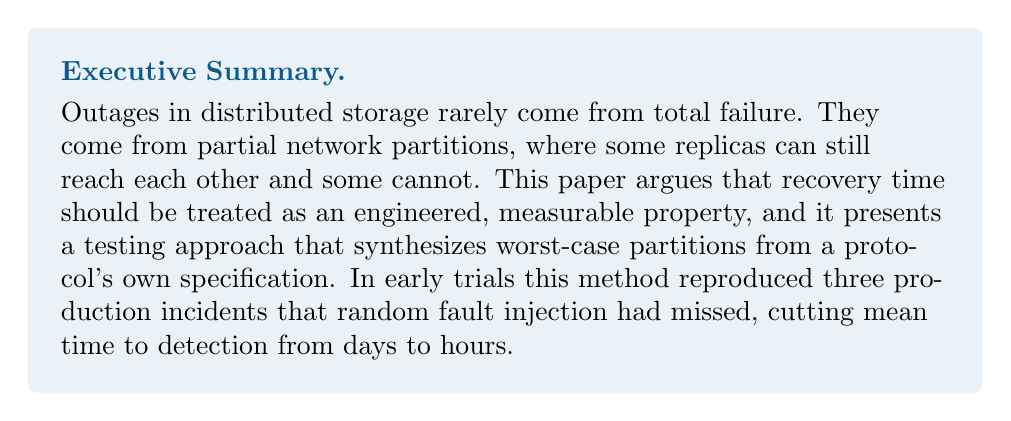
\begin{tikzpicture}
  \node[fill=panel, rounded corners=3pt, inner sep=12pt, text width=\dimexpr\textwidth-24pt\relax] {
    \textbf{\color{accent}Executive Summary.}\\[0.3em]
    Outages in distributed storage rarely come from total failure. They come from
    partial network partitions, where some replicas can still reach each other and
    some cannot. This paper argues that recovery time should be treated as an
    engineered, measurable property, and it presents a testing approach that
    synthesizes worst-case partitions from a protocol's own specification. In
    early trials this method reproduced three production incidents that random
    fault injection had missed, cutting mean time to detection from days to hours.
  };
\end{tikzpicture}

\section{The Problem}
Reliability engineering has matured around the assumption that faults are
symmetric: a link is either up or down for both endpoints. Real infrastructure
violates this assumption constantly through misconfigured firewalls, route
flaps, and one-way congestion. The result is a class of outages that pass every
test yet fail in production.

\section{Our Approach}
We treat each replication protocol as a formal state machine and search for the
connectivity patterns that maximize recovery latency. Because the search is
guided by the specification rather than by random sampling, it concentrates
effort on the faults that actually matter. The output is a small suite of
reproducible, worst-case scenarios that teams can add to their continuous
integration pipeline.

\section{Results and Recommendations}
Across three storage systems, specification-guided injection surfaced stalls
that had survived months of random testing. We recommend that operators adopt
recovery-time objectives as first-class service level indicators and validate
them against synthesized partial partitions before every release.

\end{document}
